\section{Using CIG Code from Git}

\begin{frame}[plain,noframenumbering]
 \vfill
 \begin{center}
  \LARGE \color{solarizedAccent} Using CIG Code from Git
 \end{center}
 \vfill
\end{frame}

\begin{frame}
 \frametitle{Using CIG Code from Git(Hub)}

 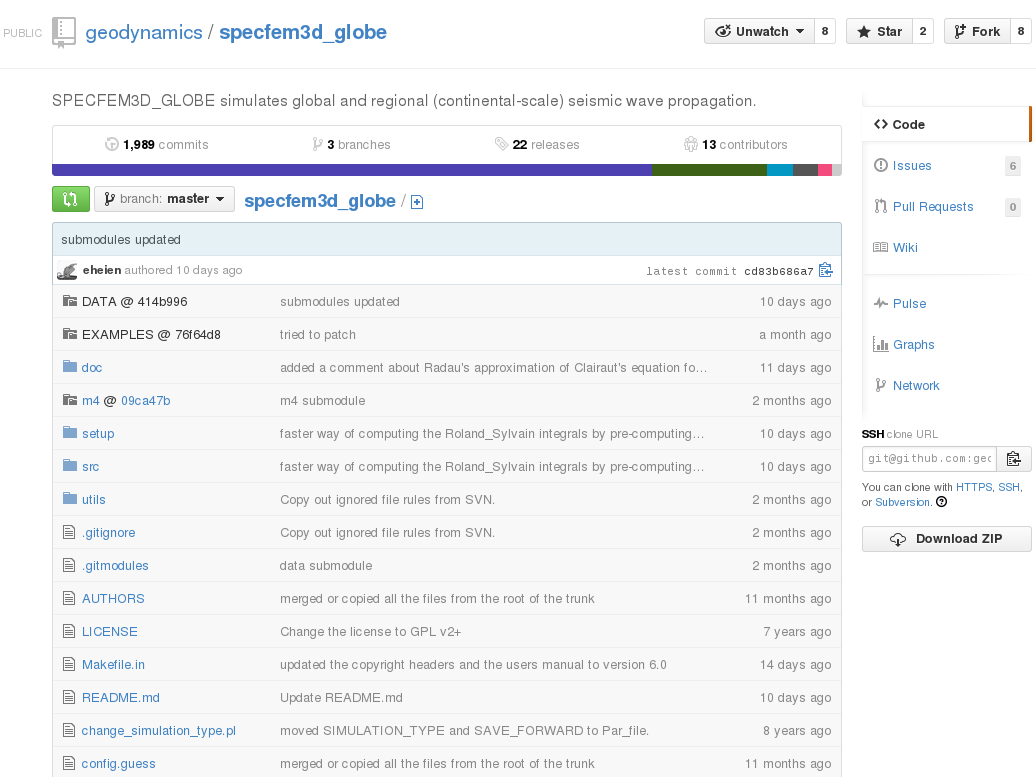
\includegraphics[height=\textheight,width=\textwidth,keepaspectratio]{github}
\end{frame}

\begin{frame}[fragile]
 \frametitle{Using CIG Code from Git}

 \begin{block}{Cloning Stable Code}
  \begin{semiverbatim}
$ git clone \alert<2>{-{}-recursive} \\
   https://github.com/geodynamics/specfem3d_globe.git
Cloning into `specfem3d_globe'...
remote: Reusing existing pack: 20478, done.
remote: Counting objects: 59, done.
remote: Compressing objects: 100% (59/59), done.
done.
Checking out files: 100% (701/701), done.
...
\end{semiverbatim}
 \end{block}
\end{frame}

\begin{frame}[fragile]
 \frametitle{Using CIG Code from Git}

 \begin{block}{Cloning Development Code}
  \begin{semiverbatim}
$ git clone -{}-recursive \alert{-{}-branch devel} \\
   https://github.com/geodynamics/specfem3d_globe.git
Cloning into `specfem3d_globe'...
remote: Reusing existing pack: 20478, done.
remote: Counting objects: 59, done.
remote: Compressing objects: 100% (59/59), done.
done.
Checking out files: 100% (701/701), done.
...
\end{semiverbatim}
 \end{block}
\end{frame}

\begin{frame}[fragile]
 \frametitle{Using CIG Code from Git}

 \begin{block}{Switching Branches}
  \begin{semiverbatim}
# Create branch tracking upstream
$ git branch -{}-track devel origin/devel
Branch origin/devel set up to track local branch \makebox[0.85\width][l]{devel}
# Switch to branch
$ git checkout devel
Switched to branch `devel'
Your branch is up-to-date with `origin/devel'.
\end{semiverbatim}
  Shortcut:
  \begin{semiverbatim}
# Create and switch to branch devel
$ git checkout \alert<3>{-{}-track} \alert<2>{-b devel} origin/devel
Branch origin/devel set up to track local branch \makebox[0.85\width][l]{devel}
Switched to branch `devel'
\end{semiverbatim}
 \end{block}
\end{frame}

\begin{frame}[fragile]
 \frametitle{Using CIG Code from Git}

 \begin{block}{Fetching Updates}
  \begin{semiverbatim}
$ git fetch \only<2>{origin}
remote: Counting objects: 85, done.
remote: Compressing objects: 100% (85/85), done.
remote: Total 85 (delta 37), reused 2 (delta 0)
Unpacking objects: 100% (85/85), done.
From https://github.com/geodynamics/specfem3d_globe
   c45b60b..f218984  devel      -> origin/devel
\end{semiverbatim}
 \end{block}
\end{frame}

\begin{frame}[fragile]
 \frametitle{Using CIG Code from Git}

 \begin{block}{Merge Updates}
  \begin{semiverbatim}
$ git merge \only<2>{origin/master}
Updating c45b60b..f218984
Fast-forward
...
\end{semiverbatim}
 \end{block}
\end{frame}
